\subsection{Differential-Mode \& Common-Mode Gain}

A sine wave centered at $0$\si{\volt} with amplitude $100$\si{\milli\volt} and frequency $1$\si{\mega\hertz} is applied to $v_{in}$ as indicated by the differential amplifier circuit schematic. 
The oscilloscope displayed the following waveforms for $V_{out+}$ and $V_{out-}$.

\FloatBarrier

\begin{figure}[h!]
	\centering
	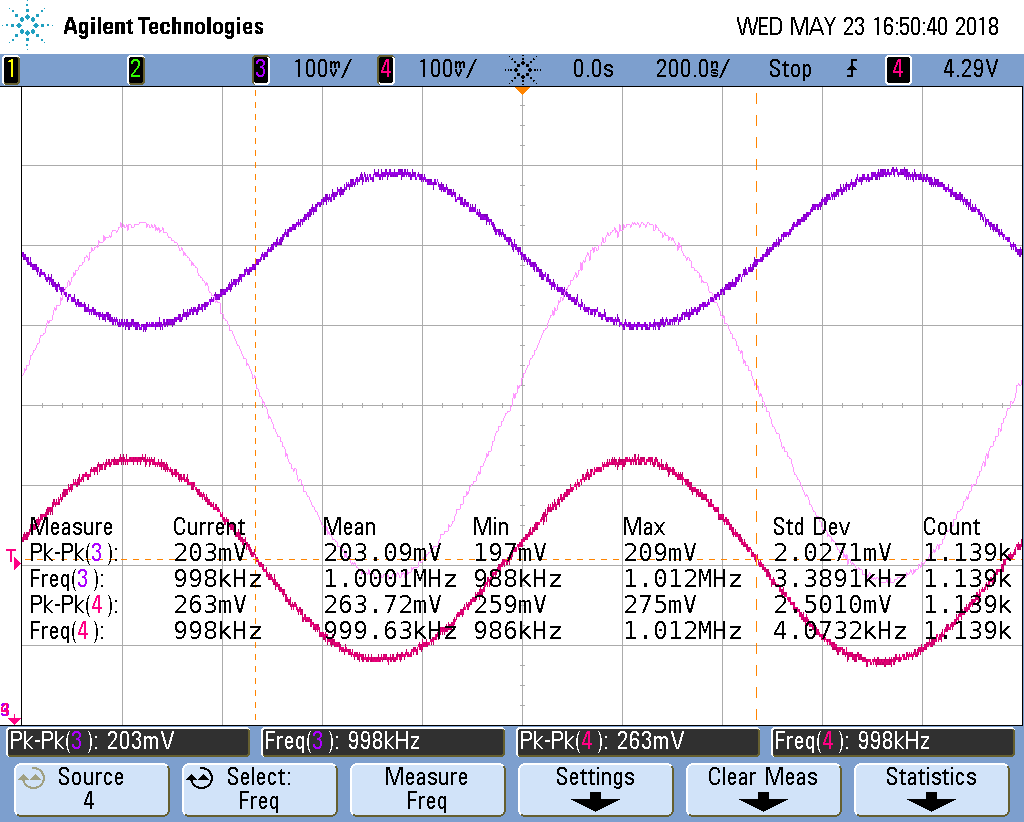
\includegraphics[scale=0.50]{./images/scope_5}
	\caption{$V_{out+}$ (4), $V_{out-}$ (3), and $V_{out+} - V_{out-}$ for $100$\si{\milli\volt} input at $1$\si{\mega\hertz}}
	\label{fig:scope_5}
\end{figure}

\FloatBarrier

As expected, $V_{out+}$ and $V_{out-}$ are $180$ degrees out of phase.
The peak-to-peak amplitudes of $V_{out+}$ and $V_{out-}$ are $263$ and $203$\si{\milli\volt}, respectively.
By taking the difference of the amplitudes, $V_{out+} - V_{out-} = 466$\si{\milli\volt} peak-to-peak. \\

The voltage applied to $V_{in-}$ has an ac amplitude of $100$\si{\milli\volt}.
The voltage applied to $V_{in+}$ has no ac component.
From these input signals, the differential-mode component of the input $v_{in(dm)} = v_{in+} - v_{in-} = -100$\si{\milli\volt} amplitude or $200$\si{\milli\volt} peak-to-peak.
The common-mode component of the input $v_{in(cm)} = \frac{1}{2}(v_{in+} + v_{in-}) = 50$\si{\milli\volt} amplitude or $100$\si{\milli\volt} peak-to-peak. \\

\subsection{Clamping \& Distortion}

\FloatBarrier

\begin{figure}[h!]
	\centering
	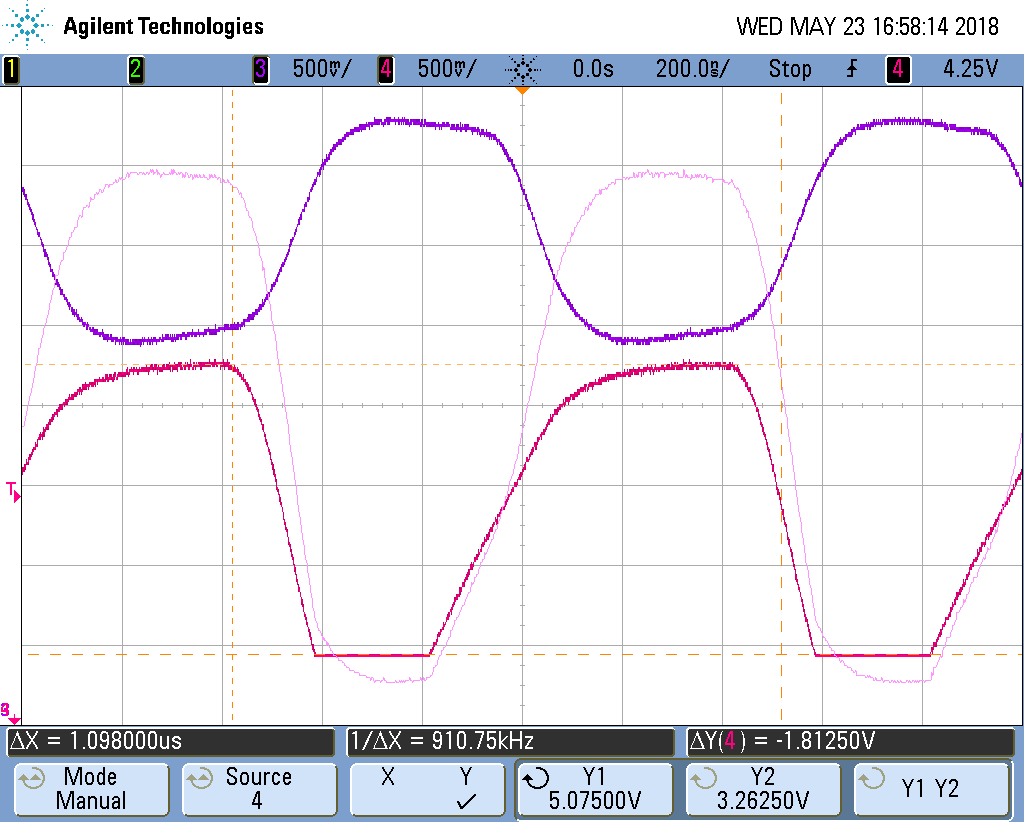
\includegraphics[scale=0.50]{./images/scope_7}
	\caption{Measured maximum signal swing of $V_{out+}$ from a 2\si{\volt} p/p input at 1MHz}
	\label{fig:scope_7}
\end{figure}

\FloatBarrier

\begin{figure}[h!]
	\centering
	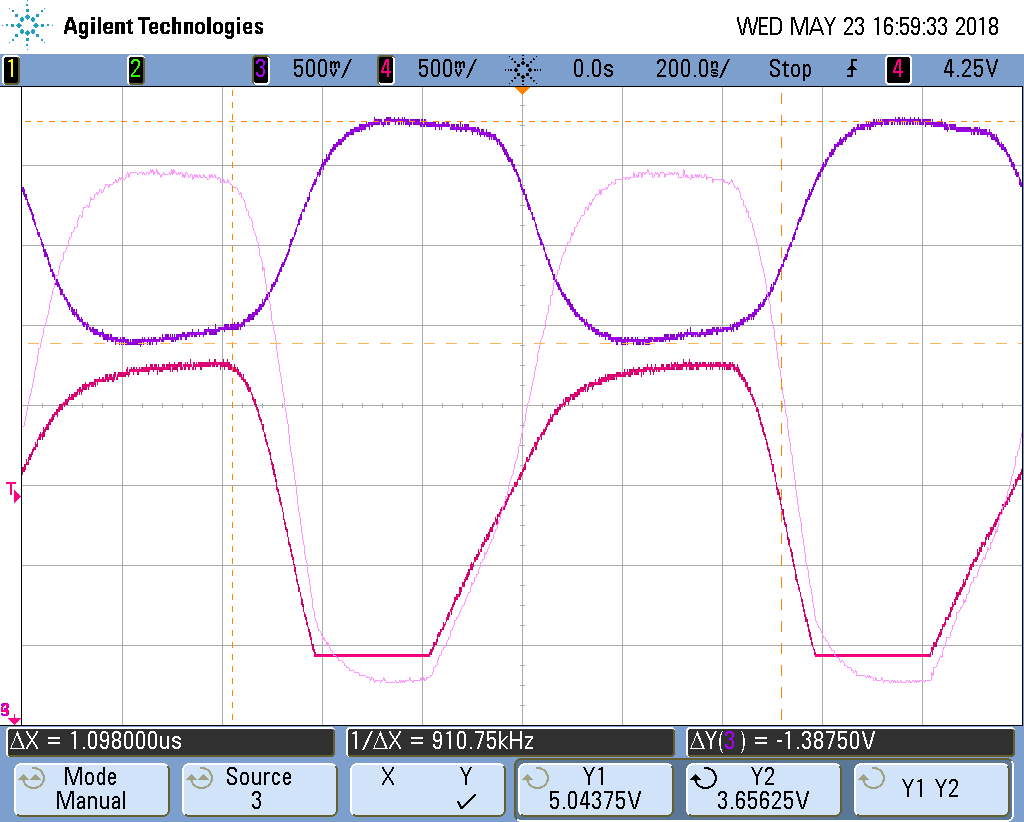
\includegraphics[scale=0.50]{./images/scope_8}
	\caption{Measured maximum signal swing of $V_{out-}$ from a 2\si{\volt} p/p input at 1MHz}
	\label{fig:scope_8}
\end{figure}

\FloatBarrier

From the cursors in (\ref{fig:scope_7}), $V_{out+}$ ranges from 5.075 to 3.262 \si{\volt}, resulting in a swing of 1.81\si{\volt}.
Similarly, the cursors in (\ref{fig:scope_8}) reveal a range of 1.38\si{\volt} for $V_{out-}$.
Thus, the voltage range for the signal $V_{out+} - V_{out-}$ is the sum of these two ranges, or 3.19\si{\volt}.
From these parameters, an input signal that will avoid clipping should have an amplitude lower than 3.19\si{\volt} / $A_{dm} \approx 1.5$ \si{\volt}.
